\section{EODP-TS-ISM. Instrument Module}
\label{sec:ism}

\subsection{Objective}
The test validates the Instrument Module.
The ISM converts the input TOA spectral radiances into digital numbers in three stages \cite{atbd}.
\begin{itemize}
\item Optical stage. Spectral integration with the ISRF, conversion to irradiance and application of the system MTF.
\item Detection stage. Conversion to photons and electrons, PRNU, dark signal and bad or dead pixels.
\item Video chain. Conversion to volts and digitisation.
\end{itemize}
The test also answers two questions. Which MTF defines the system, and do the unit conversion factors reproduce the saved outputs.

\subsection{Inputs and configuration}
The input is the scene \texttt{gradient\_alt100\_act150/sgm\_toa.nc}.
It has 100 lines ALT, 150 columns ACT and 600 wavelengths from 400 to 999~nm.
The radiance grows linearly in the ACT direction.
Table~\ref{tab:ism_config} lists the main parameters of the default configuration.

\begin{table}[H]
\centering
\caption{Main ISM configuration parameters.}
\label{tab:ism_config}
\begin{tabular}{llr}
\toprule
Parameter & Symbol & Value \\
\midrule
Pixel size & $w$ & 30~\textmu m \\
Integration time & $t_{int}$ & 6.72~ms \\
Pupil diameter & $D$ & 0.150~m \\
Focal length & $f$ & 0.5262~m \\
Optical transmittance & $T_r$ & 0.99 \\
Central wavelengths & $\lambda$ & 490, 665, 865, 945~nm \\
Quantum efficiency & $QE$ & 0.8~e$^-$/ph \\
Full well capacity & $FWC$ & 420000~e$^-$ \\
Output conversion factor & $OCF$ & $5.4\times10^{-6}$~V/e$^-$ \\
ADC gain & $G$ & 0.56 \\
Bit depth & $N_{bits}$ & 12 \\
Voltage range & $V_{max}-V_{min}$ & 0.86~V \\
PRNU and DSNU factors & $k_{PRNU}$, $k_{DSNU}$ & 0.04, 0.2 \\
Bad and dead pixels & & 1.0~\%, 0.5~\% \\
\bottomrule
\end{tabular}
\end{table}

\subsection{Execution}
The script \texttt{harness/EODP-TS-ISM/test\_ism.py} runs the ISM with all the effects enabled.
It saves every intermediate output and the seven MTFs of each band.
Then it compares them with the reference outputs and generates the figures and tables of this section.

\subsection{Results}

\subsubsection{Cross-validation}
Tables~\ref{tab:ism_crossval_toa} and~\ref{tab:ism_crossval_mtf} show the maximum relative difference of every output with respect to the reference.
All the files are identical to the reference.
This includes the PRNU and the dark signal, which use random numbers with a fixed seed.

\begin{longtable}{lccccc}
\caption{ISM cross-validation of the TOA outputs. Maximum relative difference [\%] per band.}\label{tab:ism_crossval_toa}\\
\toprule
File & VNIR-0 & VNIR-1 & VNIR-2 & VNIR-3 & Result \\
\midrule
\endfirsthead
\toprule
File & VNIR-0 & VNIR-1 & VNIR-2 & VNIR-3 & Result \\
\midrule
\endhead
\texttt{ism\_toa\_isrf\_} & $0$ & $0$ & $0$ & $0$ & Pass \\
\texttt{ism\_toa\_optical\_} & $0$ & $0$ & $0$ & $0$ & Pass \\
\texttt{ism\_toa\_e\_} & $0$ & $0$ & $0$ & $0$ & Pass \\
\texttt{ism\_toa\_prnu\_} & $0$ & $0$ & $0$ & $0$ & Pass \\
\texttt{ism\_toa\_ds\_} & $0$ & $0$ & $0$ & $0$ & Pass \\
\texttt{ism\_toa\_detection\_} & $0$ & $0$ & $0$ & $0$ & Pass \\
\texttt{ism\_toa\_} & $0$ & $0$ & $0$ & $0$ & Pass \\
\bottomrule
\end{longtable}

\begin{longtable}{lccccc}
\caption{ISM cross-validation of the MTFs. Maximum relative difference [\%] per band.}\label{tab:ism_crossval_mtf}\\
\toprule
File & VNIR-0 & VNIR-1 & VNIR-2 & VNIR-3 & Result \\
\midrule
\endfirsthead
\toprule
File & VNIR-0 & VNIR-1 & VNIR-2 & VNIR-3 & Result \\
\midrule
\endhead
\texttt{Hdiff\_} & $0$ & $0$ & $0$ & $0$ & Pass \\
\texttt{Hdefoc\_} & $0$ & $0$ & $0$ & $0$ & Pass \\
\texttt{Hwfe\_} & $0$ & $0$ & $0$ & $0$ & Pass \\
\texttt{Hdet\_} & $0$ & $0$ & $0$ & $0$ & Pass \\
\texttt{Hsmear\_} & $0$ & $0$ & $0$ & $0$ & Pass \\
\texttt{Hmotion\_} & $0$ & $0$ & $0$ & $0$ & Pass \\
\texttt{Hsys\_} & $0$ & $0$ & $0$ & $0$ & Pass \\
\bottomrule
\end{longtable}


\subsubsection{Signal through the stages}
Figure~\ref{fig:ism_stages} shows the central ALT line after each stage.
The radiance after the ISRF is a straight line, as the input scene.
The MTF modifies the first and last columns. The FFT treats the image as periodic, so the bright last column is mixed with the dark first one.
The detection stage adds the stripes of the PRNU and the DSNU.
In VNIR-2 and VNIR-3 the signal reaches the full well capacity of 420000~e$^-$.
After the video chain VNIR-1, VNIR-2 and VNIR-3 saturate at 4095~DN.

\begin{figure}[H]
\centering
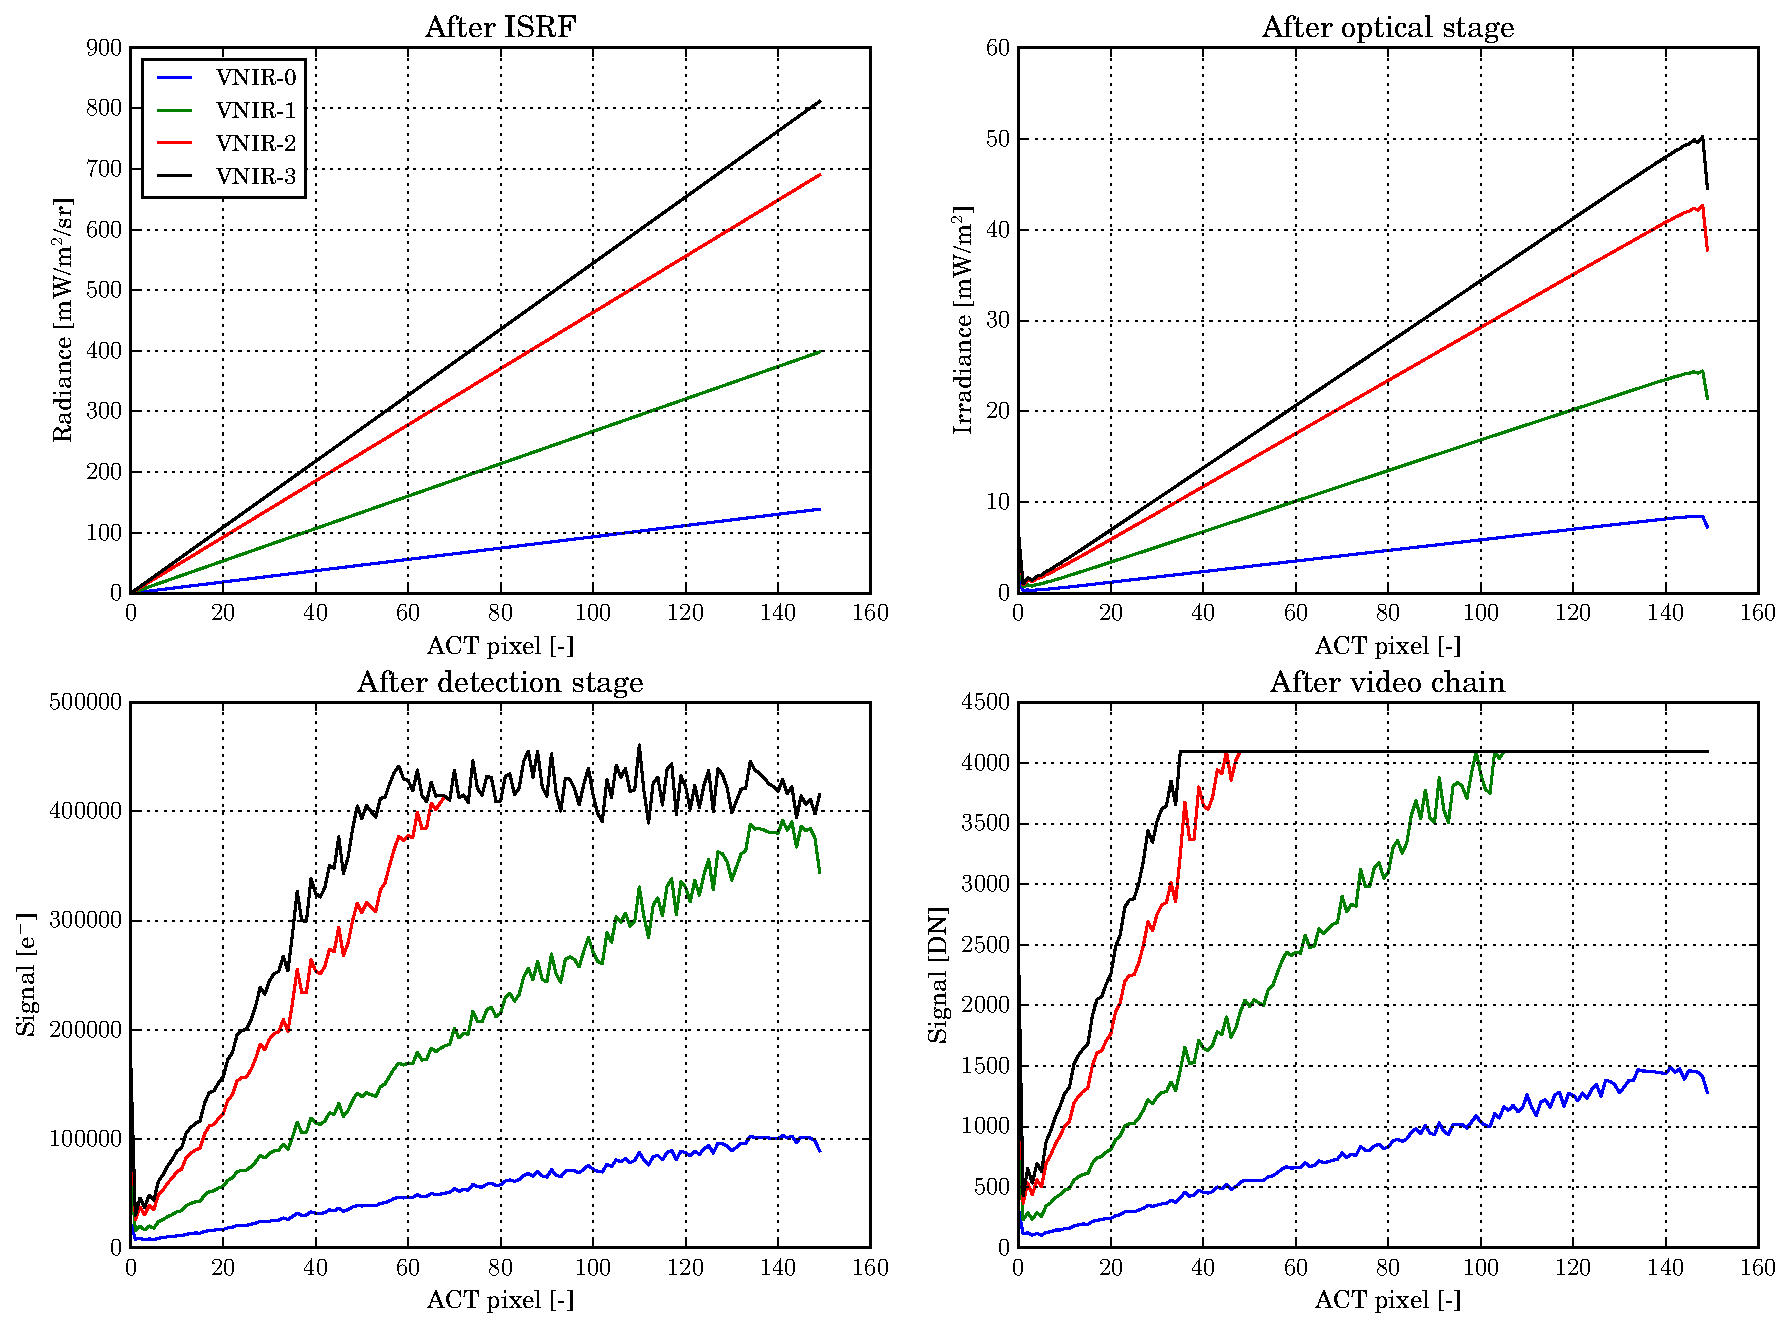
\includegraphics[width=\textwidth]{ism_stages}
\caption{ISM. Central ALT line after each stage for the four bands.}
\label{fig:ism_stages}
\end{figure}

\subsubsection{MTF}
Figures~\ref{fig:ism_mtf_0} to~\ref{fig:ism_mtf_3} show the cuts of the MTF in the ACT and ALT directions up to the Nyquist frequency.
The frequencies are normalised with the inverse of the pixel width, so Nyquist is at 0.5.
Table~\ref{tab:ism_mtf_nyquist} gives the value of each contributor at the last sample before Nyquist.

\begin{figure}[H]
\centering
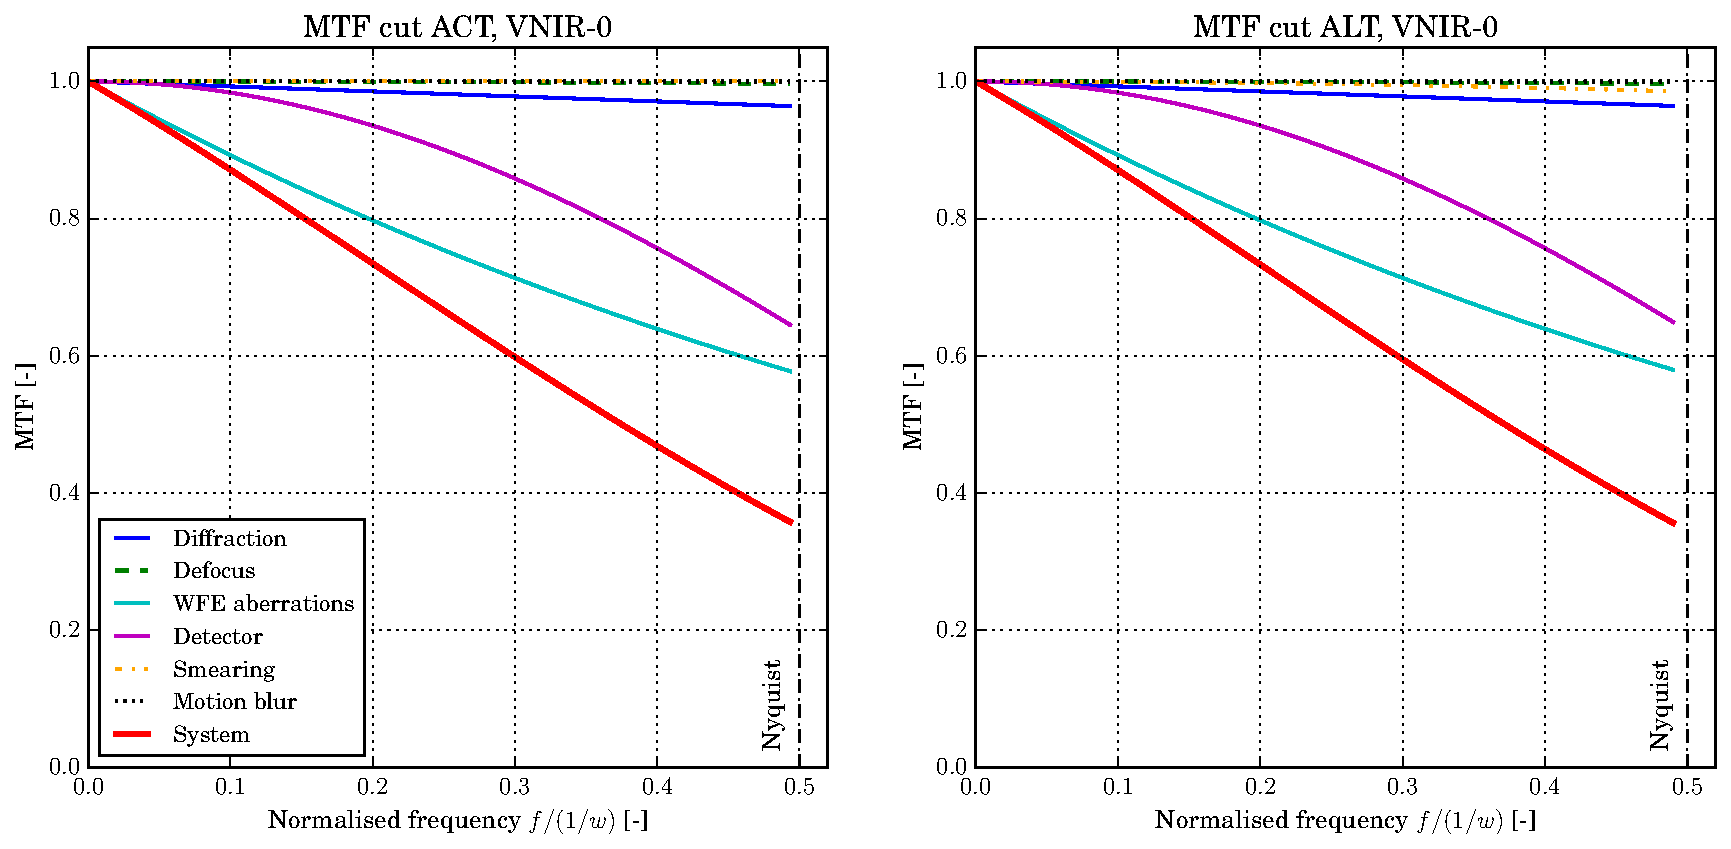
\includegraphics[width=\textwidth]{ism_mtf_VNIR-0}
\caption{ISM. MTF cuts ACT and ALT, VNIR-0.}
\label{fig:ism_mtf_0}
\end{figure}

\begin{figure}[H]
\centering
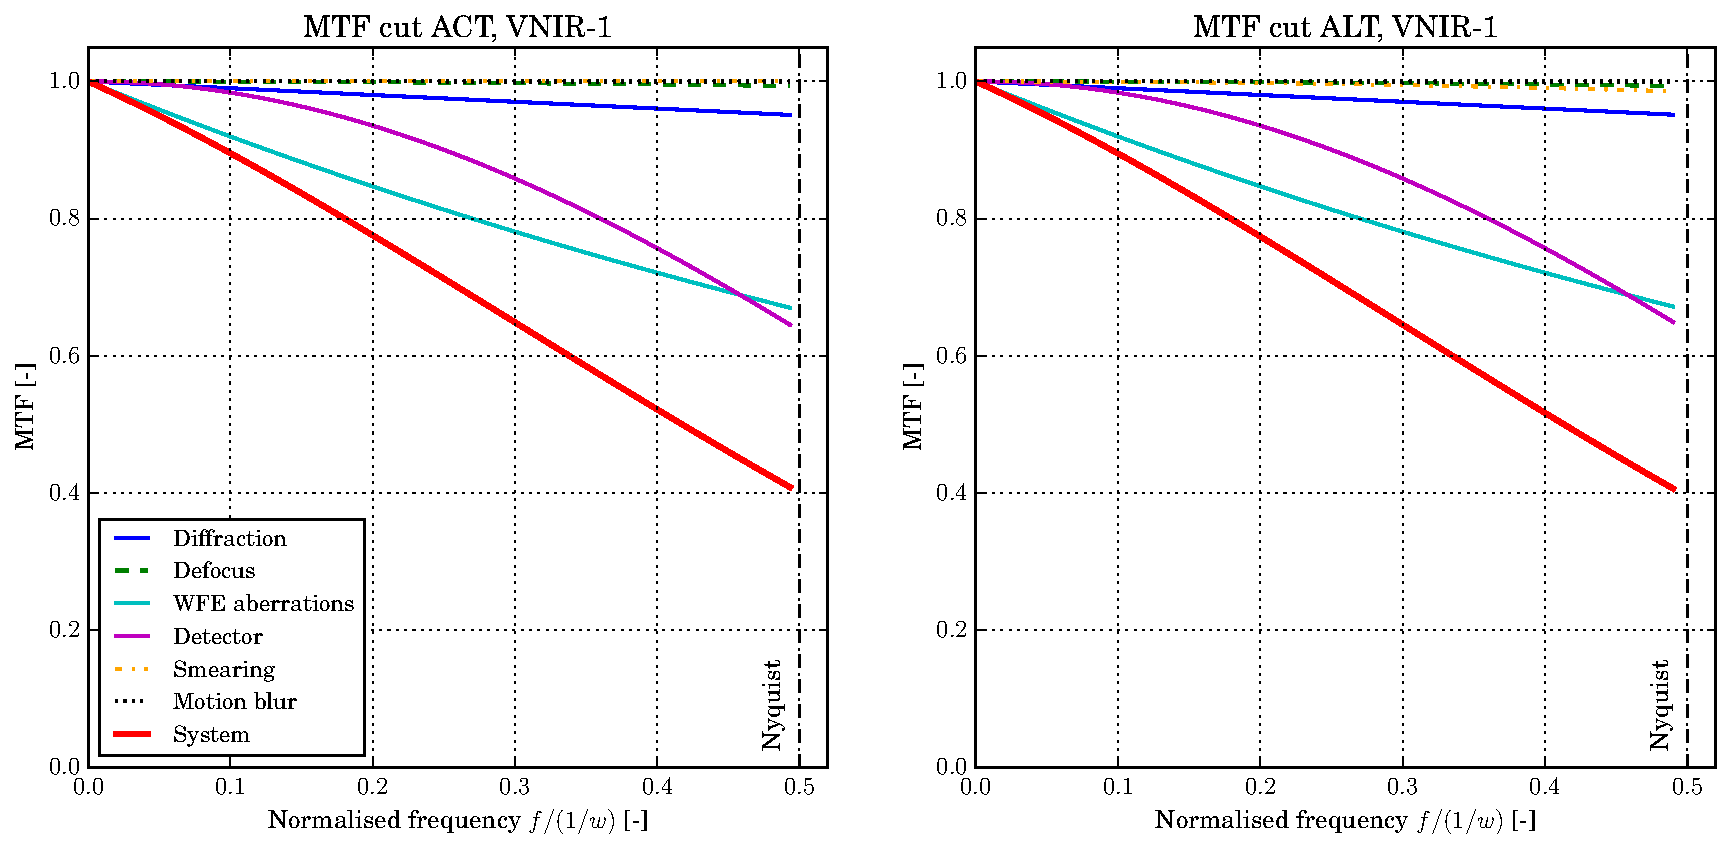
\includegraphics[width=\textwidth]{ism_mtf_VNIR-1}
\caption{ISM. MTF cuts ACT and ALT, VNIR-1.}
\label{fig:ism_mtf_1}
\end{figure}

\begin{figure}[H]
\centering
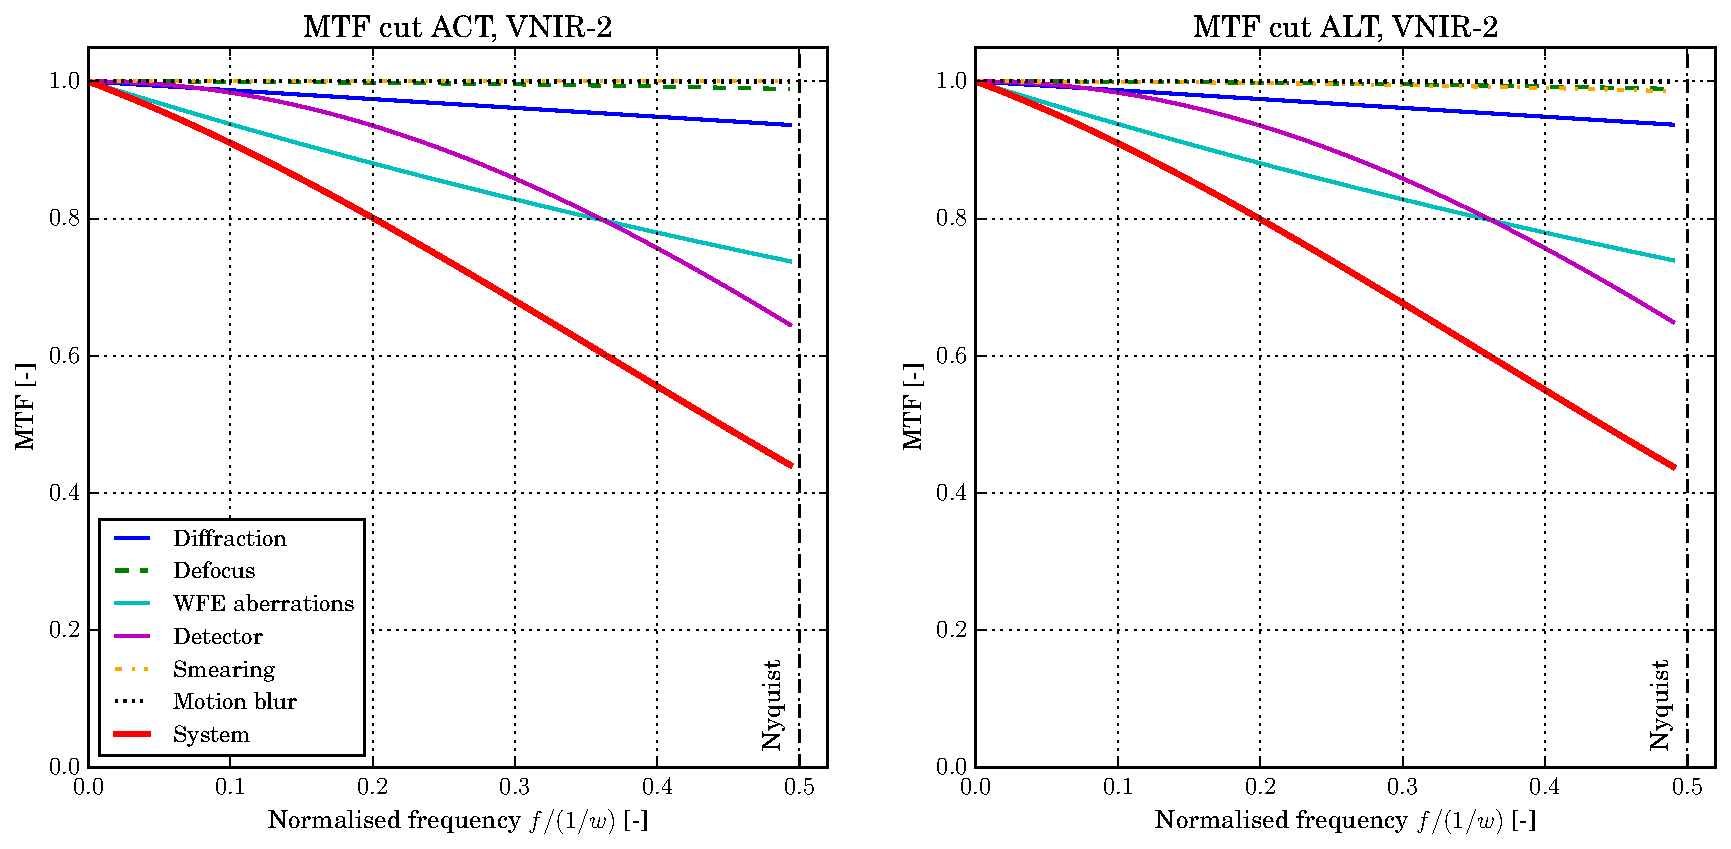
\includegraphics[width=\textwidth]{ism_mtf_VNIR-2}
\caption{ISM. MTF cuts ACT and ALT, VNIR-2.}
\label{fig:ism_mtf_2}
\end{figure}

\begin{figure}[H]
\centering
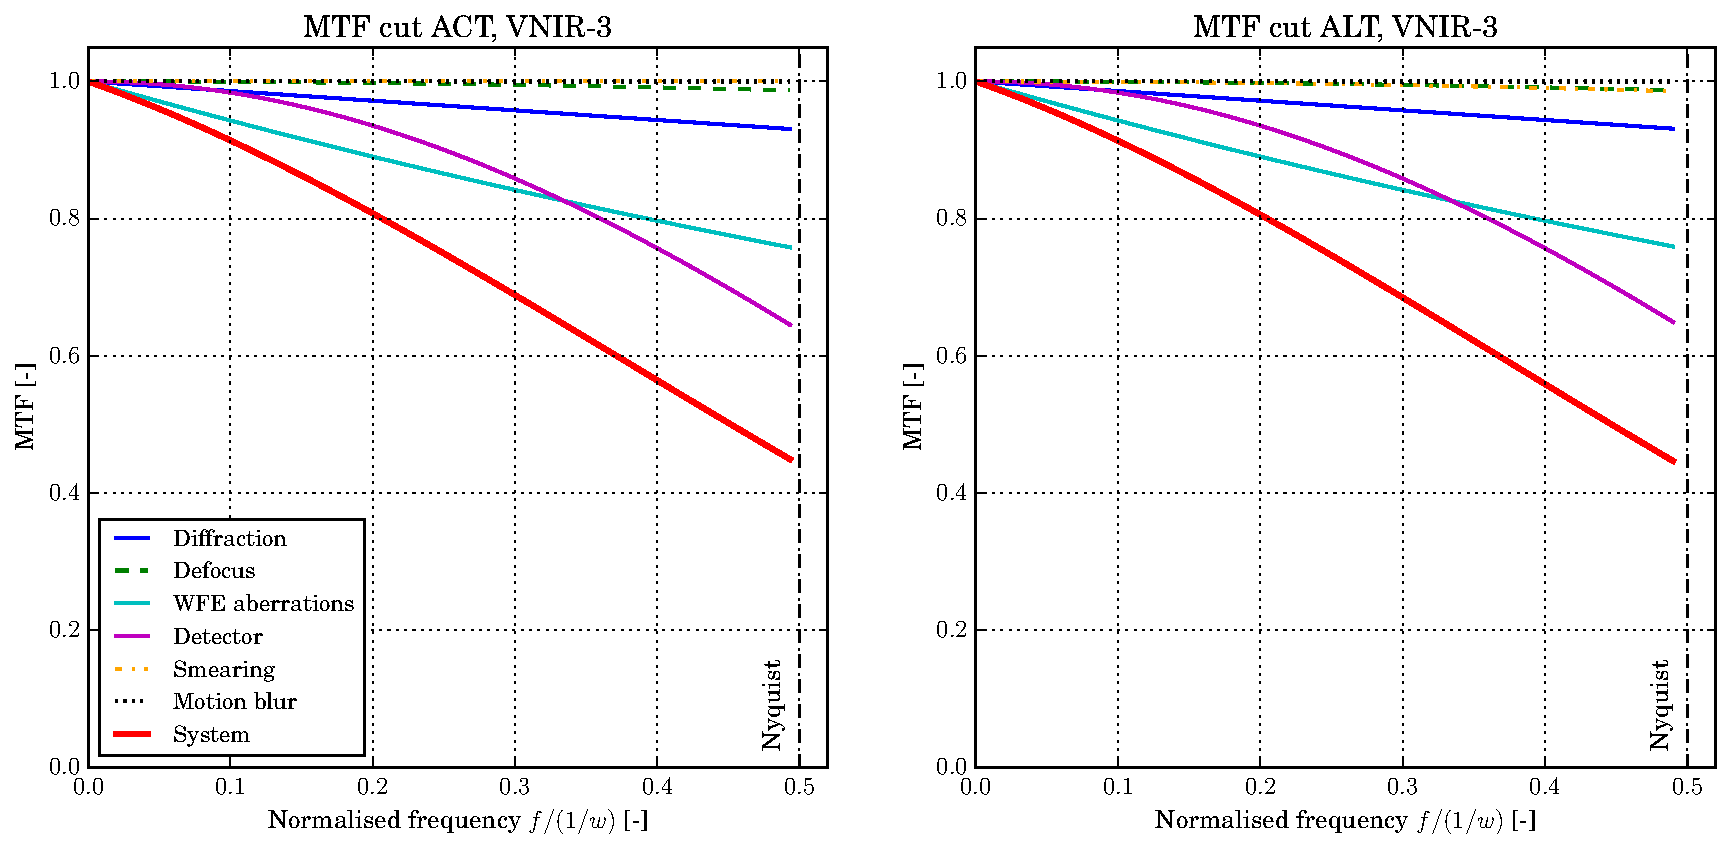
\includegraphics[width=\textwidth]{ism_mtf_VNIR-3}
\caption{ISM. MTF cuts ACT and ALT, VNIR-3.}
\label{fig:ism_mtf_3}
\end{figure}

\begin{table}[H]
\centering
\small
\caption{MTF of each contributor at the last sample before Nyquist.}
\label{tab:ism_mtf_nyquist}
\begin{tabular}{lcccccccc}
\toprule
 & \multicolumn{2}{c}{VNIR-0} & \multicolumn{2}{c}{VNIR-1} & \multicolumn{2}{c}{VNIR-2} & \multicolumn{2}{c}{VNIR-3} \\
MTF & ACT & ALT & ACT & ALT & ACT & ALT & ACT & ALT \\
\midrule
Diffraction & 0.964 & 0.964 & 0.951 & 0.951 & 0.936 & 0.937 & 0.931 & 0.931 \\
Defocus & 0.996 & 0.996 & 0.993 & 0.993 & 0.989 & 0.989 & 0.987 & 0.987 \\
WFE aberrations & 0.577 & 0.580 & 0.670 & 0.672 & 0.738 & 0.739 & 0.758 & 0.759 \\
Detector & 0.645 & 0.649 & 0.645 & 0.649 & 0.645 & 0.649 & 0.645 & 0.649 \\
Smearing & 1.000 & 0.986 & 1.000 & 0.986 & 1.000 & 0.986 & 1.000 & 0.986 \\
Motion blur & 1.000 & 1.000 & 1.000 & 1.000 & 1.000 & 1.000 & 1.000 & 1.000 \\
System & 0.358 & 0.356 & 0.408 & 0.406 & 0.441 & 0.438 & 0.449 & 0.447 \\
\bottomrule
\end{tabular}

\end{table}

\subsubsection{Unit conversion at the central pixel}
Each conversion of the ISM is a scalar factor for a given band.
Table~\ref{tab:ism_units_factors} lists the factors.
They are
\begin{align}
I &= L \cdot T_r \frac{\pi}{4}\left(\frac{D}{f}\right)^2, &
N_{ph} &= I \cdot \frac{A_{pix}\, t_{int}\, \lambda}{h c}, &
N_e &= N_{ph} \cdot QE, \\
V &= N_e \cdot OCF \cdot G, &
DN &= \mathrm{round}\left( V \cdot \frac{2^{N_{bits}}-1}{V_{max}-V_{min}} \right). & &
\end{align}
The irradiance is converted from mW to W before the conversion to photons.
The factors are applied to the radiance of the central pixel [50, 75] of \texttt{ism\_toa\_isrf}.
The result is compared with the two outputs that the code saves in these units. They are the electrons of \texttt{ism\_toa\_e} and the digital numbers of \texttt{ism\_toa}.
Irradiance, photons and volts are not saved.
Table~\ref{tab:ism_units_check} shows the comparison.

\begin{table}[H]
\centering
\small
\caption{Unit conversion factors per band. The two largest factors of each band are in bold.}
\label{tab:ism_units_factors}
\begin{tabular}{llcccc}
\toprule
Step & Units & VNIR-0 & VNIR-1 & VNIR-2 & VNIR-3 \\
\midrule
Radiance $\rightarrow$ irradiance & [sr] & $6.32\times10^{-2}$ & $6.32\times10^{-2}$ & $6.32\times10^{-2}$ & $6.32\times10^{-2}$ \\
Irradiance $\rightarrow$ photons & [ph m$^2$/mW] & $\mathbf{1.49\times10^{4}}$ & $\mathbf{2.02\times10^{4}}$ & $\mathbf{2.63\times10^{4}}$ & $\mathbf{2.88\times10^{4}}$ \\
Photons $\rightarrow$ electrons & [e$^-$/ph] & $8.00\times10^{-1}$ & $8.00\times10^{-1}$ & $8.00\times10^{-1}$ & $8.00\times10^{-1}$ \\
Electrons $\rightarrow$ volts & [V/e$^-$] & $3.02\times10^{-6}$ & $3.02\times10^{-6}$ & $3.02\times10^{-6}$ & $3.02\times10^{-6}$ \\
Volts $\rightarrow$ DN & [DN/V] & $\mathbf{4.76\times10^{3}}$ & $\mathbf{4.76\times10^{3}}$ & $\mathbf{4.76\times10^{3}}$ & $\mathbf{4.76\times10^{3}}$ \\
\bottomrule
\end{tabular}

\end{table}

\begin{table}[H]
\centering
\small
\caption{Analytic conversion at the central pixel compared with the saved outputs.}
\label{tab:ism_units_check}
\begin{tabular}{lcccc}
\toprule
Quantity & VNIR-0 & VNIR-1 & VNIR-2 & VNIR-3 \\
\midrule
Radiance $L$ [mW/m$^2$/sr] & 69.8533 & 200.3996 & 347.5041 & 408.5177 \\
Electrons, analytic from $L$ [e$^-$] & 52676.1 & 205092.4 & 462601.4 & 594119.3 \\
Electrons, \texttt{ism\_toa\_e} [e$^-$] & 52673.4 & 205082.8 & 420000.0 & 420000.0 \\
Electrons, analytic from optical TOA [e$^-$] & 52673.4 & 205082.8 & 462581.2 & 594093.7 \\
DN, analytic from $L$ [DN] & 758 & 2953 & 6661 & 8555 \\
DN, \texttt{ism\_toa} [DN] & 804 & 2985 & 4095 & 4095 \\
DN, analytic from detection TOA, saturated [DN] & 804 & 2985 & 4095 & 4095 \\
\midrule
Rel. diff. electrons [\%] & -0.005 & -0.005 & -9.209 & -29.307 \\
Rel. diff. DN [\%] & 6.069 & 1.084 & -38.523 & -52.133 \\
\bottomrule
\end{tabular}

\end{table}

The analytic values do not match the saved outputs exactly.
Some steps of the ISM change the value of the signal but not its units.
\begin{itemize}
\item The MTF is applied between the irradiance and the photons. It explains the difference of $-0.005\,\%$ in the electrons of VNIR-0 and VNIR-1. If the chain starts from the optical TOA, which already includes the MTF, the electrons match \texttt{ism\_toa\_e}.
\item The FWC limits the electrons to 420000~e$^-$. In VNIR-2 and VNIR-3 the analytic value is higher, so the saved value is the FWC.
\item The PRNU, the dark signal and the bad pixels are applied after \texttt{ism\_toa\_e}. They change the DN by $+6\,\%$ in VNIR-0 and by $+1\,\%$ in VNIR-1. If the chain starts from the detection TOA, the DN match \texttt{ism\_toa}.
\item The digitisation rounds the signal and saturates it at $2^{12}-1 = 4095$~DN. VNIR-2 and VNIR-3 are saturated at the central pixel.
\end{itemize}

The two most significant steps are the ones with the largest factors.
They are the conversion from irradiance to photons, with a factor between $1.5\times10^{4}$ and $2.9\times10^{4}$, and the conversion from volts to DN, with a factor of $4.76\times10^{3}$.
The first factor grows with the wavelength because a photon of longer wavelength carries less energy.

\subsection{Theoretical question. Which MTF defines the system?}
The system MTF is the product of the six contributors.
The contributor with the lowest value at Nyquist drives the system MTF down the most.
Table~\ref{tab:ism_mtf_nyquist} shows two dominant terms.
\begin{itemize}
\item The detector MTF is $|\mathrm{sinc}(f_n)|$. It only depends on the pixel width. At Nyquist it is close to $2/\pi \approx 0.64$ in all the bands.
\item The wavefront error MTF depends on $(W/\lambda)^2$. It is lower at short wavelengths. In VNIR-0 it is 0.58 and it is the lowest contributor. In the other bands it is between 0.67 and 0.76.
\end{itemize}
So the detector defines the system MTF in VNIR-1, VNIR-2 and VNIR-3, and the wavefront error aberrations define it in VNIR-0.
The diffraction MTF stays above 0.93. The optics cut-off frequency $D/(\lambda f)$ is between 9 and 17 times the sampling frequency $1/w$. Nyquist is then at only 3 to 6~\% of the cut-off frequency.
Defocus, smearing and motion blur are close to one. Smearing only acts in the ALT direction.
The system MTF at Nyquist is between 0.36 and 0.45. This value is high, so the system is prone to aliasing.


\textbf{EODP-TS-ISM: PASS.}
